
\documentclass[]{report}
\voffset=-1.5cm
\oddsidemargin=0.0cm
\textwidth = 480pt


\usepackage{amsmath}
\usepackage{graphicx}
\usepackage{amssymb}
\usepackage{framed}
\usepackage{multicol}
%\usepackage[paperwidth=21cm, paperheight=29.8cm]{geometry}
%\usepackage[angle=0,scale=1,color=black,hshift=-0.4cm,vshift=15cm]{background}
%\usepackage{multirow}
\usepackage{enumerate}

\usepackage{amsmath,amsfonts,amssymb}
\usepackage{color}
\usepackage{multirow}
\usepackage{eurosym}
\usepackage{framed}

%\input def.tex
%\input dsdef.tex
%\input rgb.tex

%\newcommand \la{\lambda}
%\newcommand \al{a}
%\newcommand \be{b}
\newcommand \x{\overline{x}}
\newcommand \y{\overline{y}}

\begin{document}
	
%%- http://www3.ul.ie/ramsey/Lectures/Operations_Research_2/gametheory1.pdf

\chapter{CHAPTER - GAME THEORY}
\section{3.1 The Concept of a Game}
A game is defined by
\begin{itemize}
	\item a) The set of players (at least two ”rational” players).
	\item b) The set of actions available to each player (each has at least
	two possible actions).
	\item c) A payoff function, which gives the (expected) payoff of each
	player given the actions used by the players. The (expected) payoff
	of a player does depend on the actions used by the other players.
\end{itemize}


%%- 1 / 45
%-----------------------------------------------------------%
%% \section{3.1 The Concept of a Game}
\begin{itemize}
	\item According to such a definition, roulette is not a mathematical
	game, since the expected winnings of a player only depend on how
	he/she plays.
	\item The lottery is a mathematical game. Although the probability of
	winning the jackpot is independent of the choices of other players,
	a player can maximise his/her expected reward by choosing
	combinations of numbers that other individuals do not choose
	(such an individual is not more likely to win the jackpot, but when
	he/she wins, he/she wins more on average).
\end{itemize}


%-----------------------------------------------------------%
%% 2 / 45
%===========================================================%
\section{3.2 The Matrix Form of a 2-Player Game}
\begin{itemize}
	\item Assume that each player has a finite set of actions to choose from.
	\item In the matrix form of a 2-player game, each row corresponds to an
	action of Player 1 and each column corresponds to an action of
	Player 2.
	\item Each cell of the payoff matrix is associated with a payoff vector.
	The i-th component of this vector gives the payoff to Player i.
\end{itemize}


%% 3 / 45

%===========================================================%
%% 3.2 The Matrix Form of a 2-Player Game
For example, the following describes a so called Hawk-Dove game
H D
H (-2,-2) (4,0)
D (0,4) (2,2)
For example, when Player 1 plays H and Player 2 plays D, Player 1
obtains a payoff of 4 and Player 2 obtains a payoff of 0.

%-----------------------------------------------------------%
%% 4 / 45
\section{3.2 The Matrix Form of a 2-Player Game}
In general, a 2-player matrix game can be described by
\begin{enumerate}
	\item The set of actions available to Player 1,
	A = {a1, a2, . . . , am}.
\item The set of actions available to Player 2,
	B = {b1, b2, . . . , bn}.
\item The m × n matrix of 2-dimensional vectors giving the
	payoffs of both players for each of the m × n possible
	combinations of actions. The payoff of Player k when
	Player 1 plays ai and Player 2 plays bj will be
	denoted Rk (ai
	, bj).
	
\end{enumerate}

%-----------------------------------------------------------%
%% 5 / 45
%% 3.2 The Matrix Form of a 2-Player Game
\begin{itemize}
	\item One advantage of the matrix form of a game is its simplicity.
	\item	One disadvantage is that it is assumed that players choose their
	actions simultaneously.
	\item That is to say, the actions may be
	interpreted as strategies which are chosen at the beginning of a
	game.
	\item	As we continue through this chapter, we will differentiate between
	the concept of action and the concept of strategy.
	
\end{itemize}

%-----------------------------------------------------------%
% 6 / 45
\section{Zero-sum and Constant-sum Games}
\begin{itemize}
	\item A game is said to be a constant sum game, if the sum of the
	payoffs obtained by the players is fixed, regardless of the
	combination of strategies used.
	\item	A game is said to be a zero-sum game, if the sum of payoffs
	obtained by the players is always 0, regardless of the combination
	of strategies used.
	\item A game of constant sum k is essentially the same as a zero-sum
	game. A referee could pay both of the players k/2 and require that
	they play the game in which each payoff is reduced by k/2 (this
	would be a zero-sum game).
	\item	2-player constant-sum games are games of pure conflict.
	Whatever one player gains, the other will lose.
\end{itemize}

%% 7 / 45
%==========================================================%
\section{3.3 The Extensive Form of a Game}
In many games, e.g. chess, each player makes a sequence of moves.
Such a game can be represented by a tree. Each node represents a
position (state) in which a player must make a move.
Each edge coming out of a node represents a move that the player
can make in that particular state.
Each terminal point of the tree is associated with a payoff vector.
8 / 45
%==========================================================%

\subsection{The Asymmetric Hawk-Dove Game}


\begin{figure}[h!]
\centering
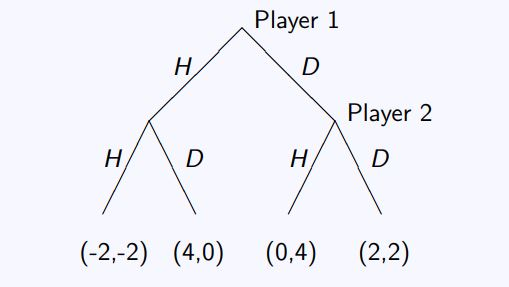
\includegraphics[width=0.7\linewidth]{images/DR5-Slide09}
\caption{}
\label{fig:DR5-Slide09}
\end{figure}


%% 9 / 45
%% The Asymmetric Hawk-Dove Game
In such a game, Player 1 first decides whether to play H and D.
After observing the decision of Player 1, Player 2 then decides
whether to play H and D.
For example, if Player 1 chooses H and Player 2 chooses D, Player
1 obtains a payoff of 4 and Player 2 obtains a payoff of 0.

\subsection{The Asymmetric Hawk-Dove Game}
%-----------------------------------------------------------%
%% 10 / 45

\begin{itemize}
\item It might appear that this game is equivalent to the matrix form of
	the Hawk-Dove given above.
\item In order to see the difference between these games, we should
	differentiate between strategies and actions.
\item In a game represented in extensive form, a strategy is a rule that
	defines which action a player should play at all the nodes where
	he/she makes a move.
\item An action is the observed behaviour resulting from such a strategy.
\end{itemize}


%-----------------------------------------------------------%
%% 11 / 45
\begin{itemize}
	\item Here Player 1 first chooses between H and D. This is her only
	choice. 
	\item Thus Player 1’s strategies correspond exactly to her
	possible actions (H and D).
	However, since Player 2 observes the move made by Player 1, he
	can condition his move on the move made by Player 1.
	\item For each of the moves made by Player 1, Player 2 has 2 possible
	moves. Hence, he has $2 \times 2 = 4$ possible strategies. These are
	listed on the following slide.
\end{itemize}


%-----------------------------------------------------------%
% 12 / 45
In the extended game described above, Player 2’s strategies are
\begin{enumerate}
	\item  H|H, H|D, i.e. play H when Player 1 plays H and
	play H when Player 1 plays D, in other words always
	play H.
	\item  H|H, D|D, i.e. take the same action as Player 1.
	\item  D|H, D|D, i.e. always play D.
	\item  D|H, H|D, i.e. play D when Player 1 plays H and
	play H when Player 1 plays D.
\end{enumerate}

In the matrix game presented earlier, Player 2 cannot condition his
action on the action made by Player 1. Hence, he only has 2
strategies corresponding to the two actions H and D.

%-----------------------------------------------------------%
%% 13 / 45
\subsection{Simultaneous Moves in Extensive Form Games}
Although the extensive form of the game is designed to describe
games in which a sequence of moves are made, they can be
adapted to describe games in which moves are made
simultaneously.
This is done using information sets. Suppose two nodes represent
states in which one player moves and that player cannot
differentiate between the states.
These two nodes are said to be in the same information set. An
information set is represented by a box.
A player may only condition an action on the information set,
he/she is presently in.

%-----------------------------------------------------------%
%% - 14 / 45


\begin{figure}[h!]
\centering
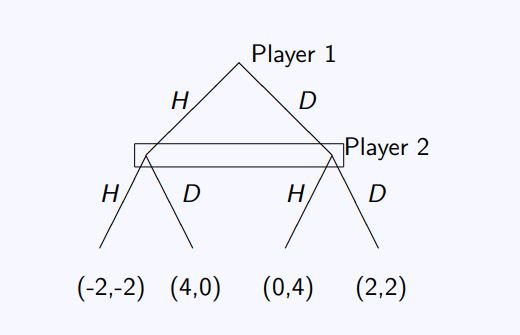
\includegraphics[width=0.7\linewidth]{images/DR5-Slide15}
\caption{}
\label{fig:DR5-Slide15}
\end{figure}
In this case both players have 2 possible strategies: H and D.

%-----------------------------------------------------------%
%% 15 / 45
\subsection{Translating from Extensive Form into Matrix Form}
In order to translate the description of a game from extensive form
to matrix form, we
\begin{enumerate}
\item  List the possible strategies of both players.
\item In the matrix describing the game, the rows
correspond to the strategies of Player 1 and the
columns correspond to the strategies of Player 2.
\item We then derive the payoff vector corresponding to
each possible strategy pair.
\end{enumerate}
%-----------------------------------------------------------%
%% 16 / 45
\begin{itemize}
	\item It should be noted that each game in extensive form has a unique
	definition as a matrix game (apart from possible differences in the
	labelling of the strategies).
\item However, there may be various games in extensive form
	corresponding to a game given in matrix form. 
\item Thus it is generally
	not possible to translate a game in matrix form into a game in
	extensive form.
\item This is unsurprising, since the extensive form of a game gives more
	detailed description of how the game is actually played.
\end{itemize}


%-----------------------------------------------------------%
%% 17 / 45
\subsection{Translating the Asymmetric Hawk-Dove Game into Matrix
Form}
\begin{itemize}
	\item Since Player 1 has 2 strategies and Player 2 has 4 strategies, the
	payoff matrix will be of dimension 2 × 4.
	\item Player 1 can play H or D.
	\item 	Player 2 can play (H|H, H|D), (H|H, D|D), (D|H, D|D) or
	(D|H, H|D). 
\end{itemize}

%-----------------------------------------------------------%
%% 18 / 45
%% \subsection{Translating the Asymmetric Hawk-Dove Game into Matrix Form}
We now consider the payoff vectors associated with each strategy
pair.
\begin{framed}
\noindent Suppose Player 1 plays H.
\begin{itemize}
	\item [(a)] If Player 2 plays (H|H, H|D) or (H|H, D|D), then both players
take the action H and the resulting payoff vector is (−2, −2).
	\item [(b)] If Player 2 plays (D|H, D|D) or (D|H, H|D), then Player 1
takes the action H and Player 2 takes the action D and the
resulting payoff vector is (4, 0).
\end{itemize}
\end{framed}

%-----------------------------------------------------------%
%19 / 45
%Translating the Asymmetric Hawk-Dove Game into Matrix Form
Now suppose Player 1 plays D.
\begin{itemize}
	\item [(a)] If Player 2 plays (D|H, D|D) or (H|H, D|D), then both players
	take the actions D and the resulting payoff vector is (2, 2).
	\item [(b)] If Player 2 plays (H|H, H|D) or (D|H, H|D), then Player 1 takes
	the action D and Player 2 takes the action H and the resulting
	payoff vector is (0, 4).
\end{itemize}

%-----------------------------------------------------------%
% 20 / 45
Translating the Asymmetric Hawk-Dove Game into Matrix
Form
It follows that the matrix form of the asymmetric game is given by
(H|H, H|D) (H|H, D|D) (D|H, D|D) (D|H, H|D)
H (-2,-2) (-2,-2) (4,0) (4,0)
D (0,4) (2,2) (2,2) (0,4)

%-----------------------------------------------------------%
%% 21 / 45
\subsection{Moves by ”Nature”}
\begin{itemize}
	\item Extensive form can also be used to describe moves by ”nature”,
	i.e. random events, the roll of a die, dealing cards.
\item Whenever nature is called to make a move at a given node, the
	edges from this node correspond to the possible results. The
	probability of each result should also be given.
\item When such a game is written in matrix form, we only consider the
	strategies that the players can use. In order to define the vector of
	expected payoffs given the combination of strategies used, we
	take expectations with respect to the moves of nature (i.e. nature
	is assumed to be ”random” or ”non-rational”).
\end{itemize}



%-----------------------------------------------------------%
%% 22 / 45
\subsection{Example}
\begin{itemize}
	\item Suppose that player 1 can first choose either A or B. Player 2 does
	not know this choice.
\item Afterwards Player 2 observes the result of a coin toss. Regardless
	of the result of the coin toss, Player 2 can play A or B.
\item If the coin toss results in heads, when both players choose the
	same action Player 1 obtains $1 from Player 2, but gives Player 2
	$1 if each chooses different actions. 
\item If the coin toss results in tails,
	when each player chooses different actions Player 1 obtains $2
	from Player 2, otherwise he gives Player 2 $2 (note this is a
	zero-sum game).
\end{itemize}


%-----------------------------------------------------------%23 / 45
\subsection{Example}
\begin{itemize}
	\item When writing the game in extensive form, we can often shift a
	move to an different position in the tree than its natural position,
	in order to make a more legible tree.
	\item	The important thing here is to correctly describe what information
	each player has when making a move.
	\item In this example, Player 1 does not know the result of the coin toss
	(or Player 2’s move).
	\item	Player 2 does not know Player 1’s move, but knows the result of
	the coin toss. Hence, Player 2’s move must come lower down the
	tree than the coin toss. We can order the moves as follows:
	nature, Player 1, Player 2.
\end{itemize}

24 / 45
Example

\begin{figure}
\centering
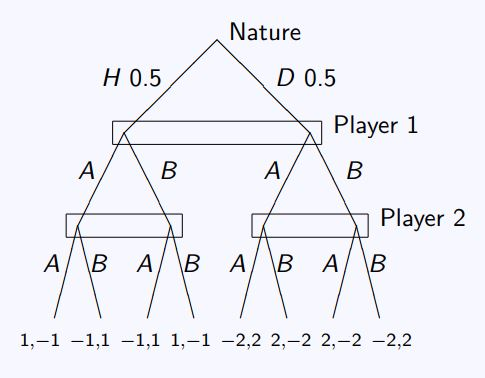
\includegraphics[width=0.7\linewidth]{images/DR5-Slide25}
\caption{}
\label{fig:DR5-Slide25}
\end{figure}

%====================================================%
25 / 45
Example
In order to describe the game in matrix form, note that Player 1
has no information regarding the coin toss or Player 2’s move. It
follows that she has 2 strategies: A and B.
Player 2 has no information regarding Player 1’s move, but knows
the result of the coin toss. Hence, his action can be made
conditional on the result of the coin toss. He has 4 strategies:
(A|H, A|T), (A|H, B|T), (B|H, B|T), (B|H, A|T).

%-----------------------------------------------------------%
26 / 45
Example
\begin{itemize}
	\item Suppose Player 1 plays A.
	\item	When Player 2 plays (A|H, A|T), i.e. always A, Player 1 wins 1 if
	the result of the coin toss was H and loses 2 if the result of the
	coin toss was tails. Player 1’s expected reward is
	0.5 × 1 − 0.5 × 2 = −0.5. Since the game is zero-sum, Player 2’s
	expected payoff is 0.5.
	\item	When Player 2 plays (B|H, B|T), i.e. always B, Player 1 loses 1 if
	the result of the coin toss was H and wins 2 if the result of the
	coin toss was tails. Player 1’s expected reward is
	0.5 × 2 − 0.5 × 1 = 0.5.
	\item	The expected rewards under all the other possible pairs of
	strategies can be calculated in a similar way.
\end{itemize}

%-----------------------------------------------------------%

27 / 45
\subsection{Example}
The matrix form of this game is given by
(A|H, A|T) (A|H, B|T) (B|H, B|T) (B|H, A|T)
A (-0.5,0.5) (1.5,-1.5) (0.5,-0.5) (-1.5,1.5)
B (0.5,-0.5) (-1.5,1.5) (-0.5,0.5) (1.5,-1.5)

%-----------------------------------------------------------%
%% 28 / 45
Extensive Forms of Games with a Continuum of Strategies
Consider the following game:
\begin{itemize}
	\item Player 1 chooses a number x between 0 and 1. Having observed
	the choice of Player 1, Player 2 chooses a number y between 0 and
	1.
	\item The payoff of Player 1 is given by R1(x, y) = 4xy − x. The payoff
	of Player 2 is given by R2(x, y) = 4xy − y.
	\item In order to depict choice from a continuum, instead of using
	branches we can use a triangle with a horizontal base. The
	strategy set is described alongside the corresponding triangle.
\end{itemize}

%-----------------------------------------------------------%
%% 29 / 45
%% Extensive Forms of Games with a Continuum of Strategies
\begin{itemize}
	\item If a move is unobserved by the next player to move, the base of the
	triangle should be enclosed in a box denoting an information set.
	\item Suppose the second player can observe whether the move of Player
	1 belongs to certain intervals. Each of these intervals corresponds
	to an information set.
	\item  The possible moves of Player 2 corresponding to each information
	set should be depicted by triangles extending out of these sets. 
\end{itemize}

%-----------------------------------------------------------%
%%  30 / 45
\subsection{Example 3.3.1}
The extensive form of the game described above is

\begin{figure}
\centering
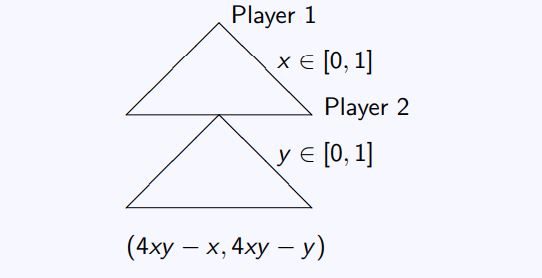
\includegraphics[width=0.7\linewidth]{images/DR5-Slide31}
\caption{}
\label{fig:DR5-Slide31}
\end{figure}

(4xy − x, 4xy − y)
%-----------------------------------------------------------%
%%  31 / 45
\subsection{The Concepts of Complete Information and Perfect
	Information}
\begin{itemize}
	\item A game is a game with complete information if both players
	know both the actions available to the other players and the
	payoffs obtained by other players under all the possible
	combinations of strategies.
\item 	In addition, if each player always knows which node of the
	extensive form of the game he/she is at when he/she has to make
	a move, then such a game is a game with perfect information.
\end{itemize}


%-----------------------------------------------------------%
%-----------------------------------------------------------%
%% 32 / 45
\subsection{The Concepts of Complete Information and Perfect
Information}
\begin{itemize}
	\item For example, chess is a game of perfect information (given a payoff
	structure of 1 point for a win, 0.5 for a draw, 0 for a loss), since
	the state of the game is always known, each player knows which
	moves are available to the opponent.
\item Bridge is definitely not a game of perfect information, as e.g. the
	bidder does not know how the cards are split between his
	opponents. 
	\item However, it may be argued that it is a game of
	complete information, since the scoring system is well defined and
	players know what others are allowed to play given their hand and
	the bidding (a full description of a strategy would however be very
	complex).
\end{itemize}


%-----------------------------------------------------------%
%% 33 / 45
\subsection{Solution of Games with Perfect Information}
\begin{itemize}
\item In games of perfect information, moves are made in succession and
each of the previous moves are known to each player.
\item Such games can be solved by recursion based on the extensive
form of the game.
\item Consider the asymmetric hawk-dove game given above. The final
move is made by Player 2. Given the move made by Player 1 (H or
D), Player 2 simply maximises his expected reward.
\item This defines Player 2’s optimal action after H and his optimal
action after D.
\end{itemize}


%-----------------------------------------------------------%
%% 34 / 45
\subsection{Solution of Games with Perfect Information}
Working backwards, Player 1 assumes that Player 2 will use his
best response to her action.
This defines the action that Player 1 should take.
It follows that there always exists a solution to a game with perfect
information. Unless at any node a player is indifferent between the
actions he/she can take, this solution will be unique.
Any vector of payoffs corresponding to the solution of such a game
is called a value of the game.
%% 35 / 45
\subsection{The Asymmetric Hawk-Dove Game}



\begin{figure}
\centering
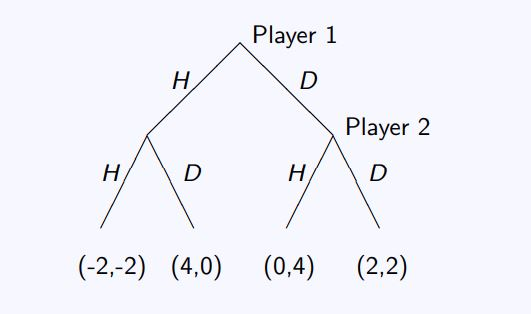
\includegraphics[width=0.7\linewidth]{images/DR5-Slide36}
\caption{}
\label{fig:DR5-Slide36}
\end{figure}

Player 2
(-2,-2) (4,0) (0,4) (2,2)

%-----------------------------------------------------------%
% 36 / 45
\subsection{Solution of Games with Perfect Information}
Suppose Player 1 has played H. Player 2 obtains -2 by playing H
and 0 by playing D. Hence, his best response to H is to play D.
Suppose Player 1 has played D. Player 2 obtains 4 by playing H
and 2 by playing D. Hence, his best response to D is H.
Now we consider the action of Player 1.

%-----------------------------------------------------------%
% 37 / 45
%% \subsection{Solution of Games with Perfect Information}
\begin{itemize}
	\item If she plays H, then Player 2 will respond by playing D. Player 1
	obtains a reward of 4.
	\item 	If she plays D, then Player 2 will respond by playing H. Player 1
	obtains a reward of 0.
	\item 	It follows that Player 1 should play H. Player 2 follows by playing
	D.
	\item 	The value of the game is (4, 0).
	
\end{itemize}

%-----------------------------------------------------------%
%% 38 / 45
\subsection{Equilibrium Path and Subgame Perfect Equilibria}
\begin{itemize}
\item The set of actions observed at a solution of an extensive form
	game with perfect information is called an equilibrium path.
\item In the Hawk-Dove game considered above, the equilibrium path is
	(H, D).
\item However, such a path does not describe how players should react to
	”mistakes”, i.e. how should individuals act off the equilibrium path.
\item An equilibrium is said to be subgame perfect, if starting from any
	node on the game tree, players play an equilibrium pair of
	strategies, i.e. an equilibrium is played in any subgame of the game
	in question.
\end{itemize}


%-----------------------------------------------------------%
% 39 / 45
% \subsection{Equilibrium Path and Subgame Perfect Equilibria}
\begin{itemize}
\item In this case, the subgame perfect equilibrium is defined by giving
the optimal response of Player 2 to each action of Player 1 and the
optimal action of Player 1.
\item These were derived during the recursive solution of the game.
Player 2 should respond to H by playing D and respond to D by
playing H. Hence, Player 2’s subgame perfect equilibrium strategy
is (D|H, H|D).
\item The subgame perfect equilibrium strategy of Player 2 is H.
If nature has moves in a game of perfect information, then each
player is assumed to maximise his/her expected reward at each
stage of the recursion procedure.

\end{itemize}

%-----------------------------------------------------------%
%%% 40 / 45
\subsection{Concepts of Pure and Mixed Strategies}
In games of perfect information, it is clear that unless a player is
indifferent between two actions, then he/she should never
randomise.
However, in games of imperfect information (e.g. when moves are
made simultaneously like rock-scissors-paper) it is clear that one
player may not want the other to ”guess” which action he/she is
going to take.
In such cases individuals choose the action they take at random,
i.e. they use a mixed strategy.

%-----------------------------------------------------------%
%%41 / 45
\subsection{Concepts of Pure and Mixed Strategies}
The matrix form of the rock-scissors-paper game is:
\begin{figure}[h!]
\centering
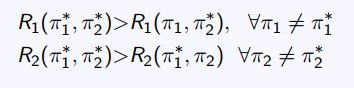
\includegraphics[width=0.7\linewidth]{images/DR7-Slide41}
\caption{}
\label{fig:DR7-Slide41}
\end{figure}

Intuitively, at equilibrium both players choose each action with a
probability of 1/3 (see tutorial sheet for details).

%-----------------------------------------------------------%
%%42 / 45
\subsection{Concepts of Pure and Mixed Strategies}
\begin{itemize}
	\item If a player always chooses the same action in a matrix game, then
	he/she is using a so called pure strategy.
	\item It is normally assumed that players choose their actions
	independently of each other (i.e. there is no communication).
	\item Later we will consider games in which players can communicate,
	i.e. the actions they take may be correlated.
\end{itemize}


%-----------------------------------------------------------%
%% 43 / 45
%% Concepts of Pure and Mixed Strategies
\begin{itemize}
	\item Suppose that in the rock-scissors-paper game, Player 1 plays rock,
	scissors and paper with probability pR, pS and pP, respectively.
\item Player 2 plays rock, scissors and paper with probability qR, qS and
	qP. The probability distribution over the set of strategy pairs is
\end{itemize}

\begin{figure}[h!]
\centering
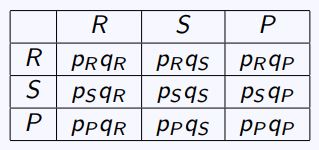
\includegraphics[width=0.5\linewidth]{images/DR5-Slide44}
\caption{}
\label{fig:DR5-Slide44}
\end{figure}

%-----------------------------------------------------------%
%% 44 / 45
%% Concepts of Pure and Mixed Strategies
When players use mixed strategies, the expected rewards of the
players can be calculated by taking expectations with respect to
the probability distribution over the set of strategy pairs. Hence,
\[R1(M1, M2)=pRqRR1(R, R) + pRqSR1(R, S) + pRqPR1(R, P) +
+pS qRR1(S, R) + pS qSR1(S, S) + pS qPR1(S, P) +
+pPqRR1(P, R) + pPqSR1(P, S) + pPqPR1(P, P)
=pRqS + pS qP + pPqR − pS qR − pPqS − pRqP.
\]

\end{document}